\section{Ranking of structural Ricardian comparative advantage }
In this section I present the results of the structural RCA ranking for both value-added exports measures and gross exports. First, I will first focus on the global view by highlighting the results of the association of the RCA ranking for gross exports and value-added exports against a country's per capita GDP. The hypothesis I focus is that country's with a higher GDP show a higher similarity between the rankings. Moreover, poorer countries production structure is such that sourcing and factor usage are more sector specific. \par Second, I will view at the structural RCA results by comparing the rankings for Belgium and Germany of forward and backward value-added exports to gross exports. In this way, I analyze whether two aspects, first whether value-added exports alter the picture of comparative advantage and whether the different perspectives of value-added exports show affect the results. 
\subsection{Structural Ricardian comparative advantage based gross exports and value-added exports}
I will discuss the choice of the assosciation measures shortly. First, I chose the rank correlation since I focus on the similarity of the ranking and the strenght of the linear association is not very interesting. Moreover I chose the kendal tau rank as it computes the similarity between the ranks based on value-added exports and gross exports for the set of countries. \par 
Moreover, kendall tau can be interpeted in a very intuitive way. To explain the intuitive interpretation, I will outline the construction of kendall's tau. The basic idea behind the measures is to count the number of different pairs for two sets of paired objects, which are based on one set of objects  \textcite{abdi2007kendall}.In the context of this thesis, this means to count the number of different country pairs for the two RCA rankings, in the following I denote this  number as $d(P_1, P_2)$, where $P_i \quad i=1,2$ indicates the order set of pairs obtained from the set of  countries. This number is normalized such that is bounded by -1 and 1, where -1 reflect the largest differences and 1 the smallest difference and its equal to 0 if the two sets show the equal order. Kendals is therefore $\tau= \frac{1/2 N(N-1) - d(P_1,P_2)} {1/2 N(N-1)}$, where the nominator $1/2 N(N-1)$ is equal to the number of pairs one can obtain from a set of $n$ objects. Further, for a pair of objects, here countrys, kendal tau has the interpretation to be equal to the difference between drawing two objects with the same order and the probability of drawing two countrys of a different order from the two rankings.
\begin{figure}
\caption{Association RCA based on VAX \& EXGR and GDP per capita }
\centering
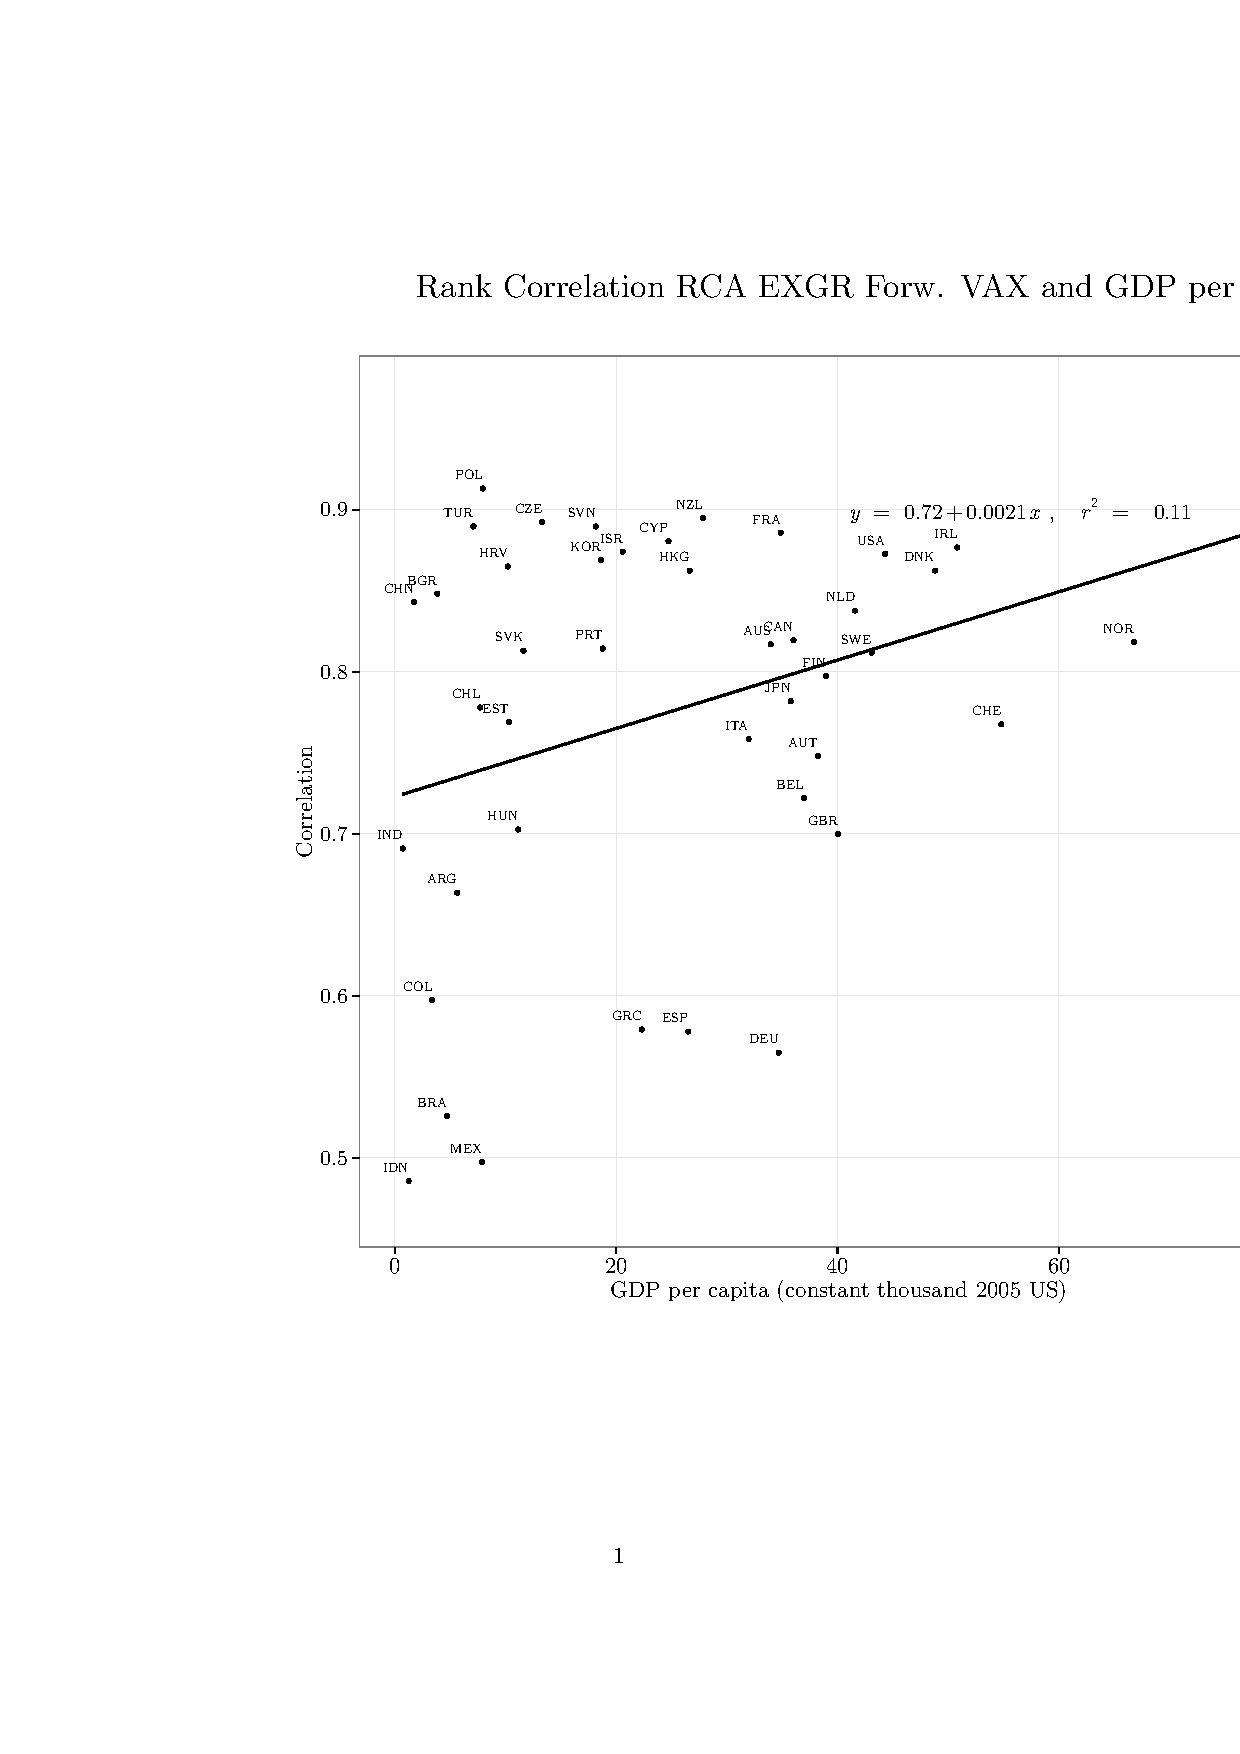
\includegraphics[width=.49 \linewidth]{./fig/spearman_fddva_std_balassa-march.tex}
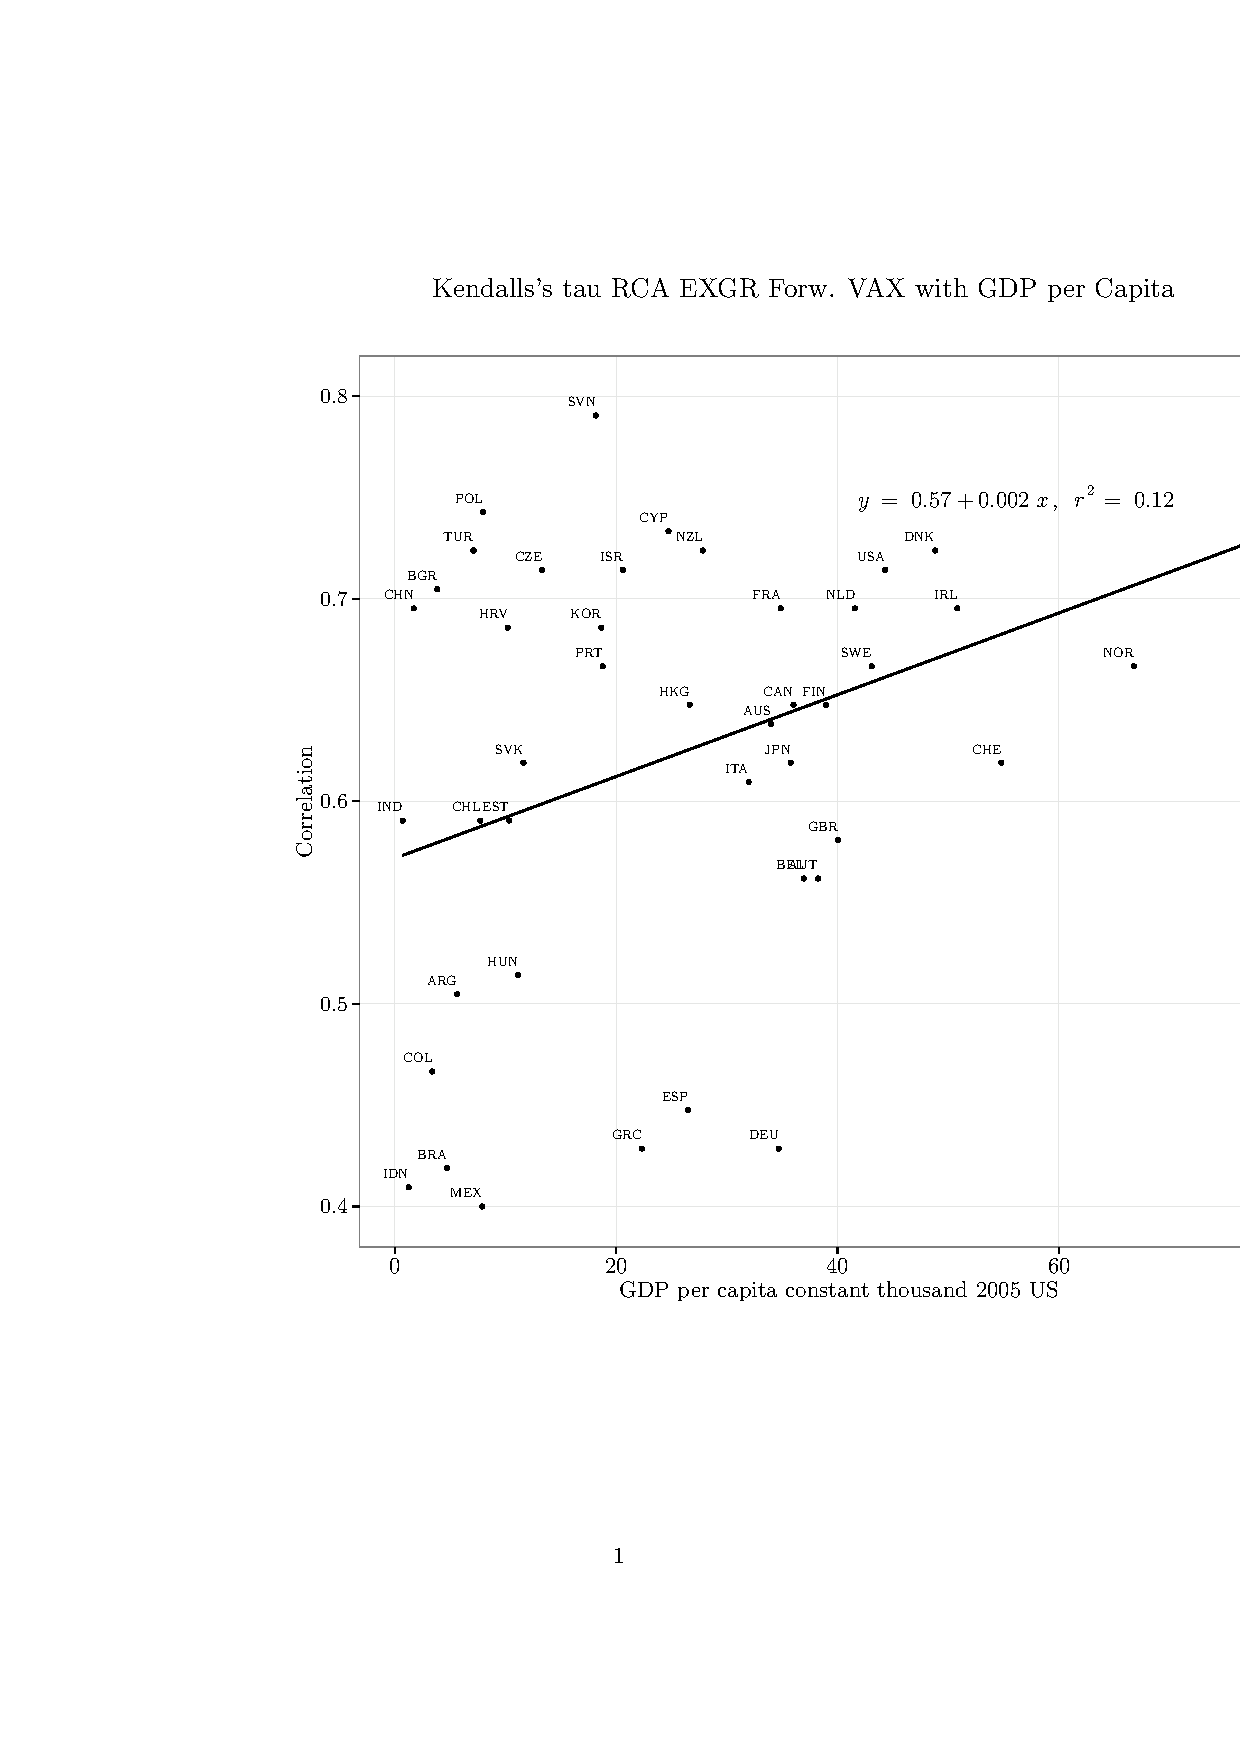
\includegraphics[width=.49 \linewidth]{./fig/kendall_fddva_exgr_std_balassa-march.tex}
 %\captionof{figure}{Another figure}
\end{figure}

\begin{figure}
\caption{Country pair RCA based on for- and backward  VAX \& EXGR }
\includegraphics[width=.5\linewidth]{./fig/back_exgr_DEU_BEL_tiva.tex}
\includegraphics[width=.5\linewidth]{./fig/forw_exgr_DEU_BEL_tiva.tex}
\end{figure}

\endinput